\documentclass[12ptpt,letterpaper]{article}
\usepackage{geometry}
\geometry{margin=1in}
\usepackage{graphicx}
\usepackage{float}
\usepackage[hidelinks]{hyperref}

\setlength{\parindent}{0pt}
\setlength{\parskip}{0.5em}

%make lists tighter
\usepackage{enumitem}
\setlist{nolistsep}

%reduce spacing before and after section
\usepackage{titlesec}
\titlespacing\section{0pt}{6pt}{0pt}

\title{Lab 1 - PECARN TBI Data, STAT 214, Spring 2026}

\author{Anonymous}

\begin{document}
\maketitle



\section{Introduction}\label{introduction}

Traumatic brain injury (TBI) is a leading cause of death and disability among children. In the emergency department, clinicians must quickly identify which pediatric head trauma patients require a computed tomography (CT) scan to detect intracranial injury. CT scans are highly sensitive but expose children to ionizing radiation, which carries long-term cancer risk---particularly in young children, whose developing brains are more radiosensitive. The clinical decision rule developed by Kuppermann et al.\ \cite{kuppermann2009} for the Pediatric Emergency Care Applied Research Network (PECARN) aims to identify children at very low risk of clinically important TBI so that unnecessary CT scans can be avoided. The rule stratifies patients by age ($<$2 vs $\ge$2 years), uses high-risk factors (GCS$\le$14, altered mental status, skull fracture signs) and medium-risk factors (vomiting, LOC, severe injury mechanism, severe headache, etc.), and recommends either obtaining a CT (high-risk) or considering CT or observation (medium-risk). Patients with no risk factors are classified as very low risk.

The purpose of this report is to perform exploratory data analysis and preprocessing on the PECARN TBI public use dataset. We examine data quality, clean the data according to documented conventions, and conduct a deeper exploration focused on \emph{relationships} between variables---how predictors interact, how age modifies predictor effects, and how compound risk accumulates. We then implement three classification models---the PECARN clinical decision rule, logistic regression, and a random forest---to predict CT recommendation outcomes, and assess their interpretability and stability. The remainder of this report is organized as follows: Section~2 describes the data, cleaning, and relationship-focused exploration; Section~3 presents three substantive findings (interactions, compound risk, model convergence), a reality check, and a stability check; Section~4 details our modeling approach; Section~5 discusses limitations and implications; Section~6 concludes. Throughout, we ground our analyses in the domain context of pediatric emergency care and the clinical stakes of head trauma decision-making.


\section{Data}\label{data}

The dataset consists of 43,399 pediatric patients (under 18 years) evaluated for head trauma at 25 PECARN emergency departments. It contains 125 variables covering patient demographics, injury mechanism, signs and symptoms (e.g., loss of consciousness, vomiting, headache), Glasgow Coma Scale components, and outcomes including CT results and clinically important TBI (ciTBI). This data is directly relevant to the domain problem: we use it to understand which clinical features predict positive CT findings and to evaluate whether the PECARN rule and alternative models can reliably identify children who need imaging versus those who can forego it.

\subsection{Data Collection}\label{data-collection}

Per the study documentation, trained site investigators and emergency physicians recorded patient history, injury mechanism, and clinical signs on standardized forms before imaging results were known. Data were collected prospectively; patients presented within 24 hours of head trauma. This prospective design reduces recall bias and ensures that predictor variables were recorded independently of outcome. The multi-site design (25 EDs) improves generalizability but introduces potential site-level variation in both patient populations and data entry practices. Site-level differences in CT utilization rates, patient demographics, or injury mechanisms could affect our findings; we did not stratify by site in this analysis, but such stratification could reveal heterogeneity. The study excluded children with trivial injury mechanisms (ground-level falls or walking into stationary objects with no signs/symptoms beyond scalp abrasions); our cohort therefore represents a selected population with at least some clinical concern, which may explain the non-negligible PosCT rate (5--6\%) among imaged patients.

The variables vary widely in their measurement scales: binary indicators (e.g., vomiting yes/no), ordinal categories (e.g., injury severity: low/moderate/high), and numeric values (e.g., age in months, GCS total). Many variables have conditional structure: for example, duration of loss of consciousness (LocLen) is only recorded when LOC is reported, and headache severity (HASeverity) applies only when headache is present. This creates structured missingness that must be handled appropriately---distinguishing ``not applicable'' from true missingness is important for interpretation. The documentation explicitly encodes these distinctions (e.g., code 92 for ``not applicable''), which we leverage during cleaning.

\subsection{Data Cleaning}\label{data-cleaning}

\textbf{Missing value codes.} The documentation specifies that missingness is encoded numerically: 91 (pre-verbal/non-verbal), 92 (not applicable), 99 (unknown/refused), 90 (other), and sometimes $-1$. We replace all such codes with NaN so that standard missing-value handling applies. This affects 81 columns. The rationale is that for downstream modeling and EDA, we need a consistent representation of missingness; treating 92 as ``not applicable'' is conceptually distinct from ``unknown'' (99), but for most analyses we treat both as missing unless the variable's semantics require otherwise. We did not retain ``not applicable'' as a distinct category for variables where it might carry information (e.g., Amnesia\_verb = 91 for pre-verbal children indicates the child cannot answer); we chose simplicity and consistency. For example, PosCT and EDCT use 92 when no CT was performed---in that case, we have no outcome for modeling and exclude such rows from the analysis cohort.

\textbf{Consistency issues.} We identified two types of inconsistencies. First, in 56 rows the sum of GCS components (eye, verbal, motor) does not equal the recorded GCSTotal. GCS is defined as the sum of three components (each scored 1--6 for verbal, 1--5 for eye, 1--6 for motor); any mismatch suggests data entry or transcription error. We flag these rows but do not drop them, as the recorded GCSTotal may still be clinically valid (e.g., if the components were entered incorrectly but the total was correct). Second, AgeTwoPlus (indicating $<$2 vs $\ge$2 years for PECARN rule stratification) disagrees with the age group implied by AgeInMonth in the majority of rows. For instance, a patient with AgeInMonth = 18 (1.5 years) might have AgeTwoPlus = 2 ($\ge$2 years). This may reflect that AgeTwoPlus was assigned at enrollment for study stratification, or that AgeInMonth was recorded/cleaned differently. We retain AgeTwoPlus as the primary age-group variable for PECARN-related analyses, since the rule was derived using that variable.

\textbf{Outcome variables.} PosCT (positive CT finding) is missing when CT was not performed; we restrict modeling to the subset with CT done and non-missing PosCT. We derive ciTBI (clinically important TBI) as the composite of DeathTBI, Neurosurgery, Intub24Head, or PosIntFinal, following the Kuppermann definition. ciTBI is a stricter outcome than PosCT: not all positive CT findings are clinically important. The analysis cohort for modeling (CT done, non-missing PosCT) yields 14,983 patients; the broader analysis cohort (GCS 14--15, CT or outcome available) yields 42,429 patients.

All preprocessing is in \texttt{clean.py} via \texttt{clean\_data()}. Figure~\ref{fig:eda} shows missingness and key distributions. Figure~\ref{fig:gcs} illustrates the GCS consistency check and missingness among PECARN rule variables.

\begin{figure}[H]
\centering
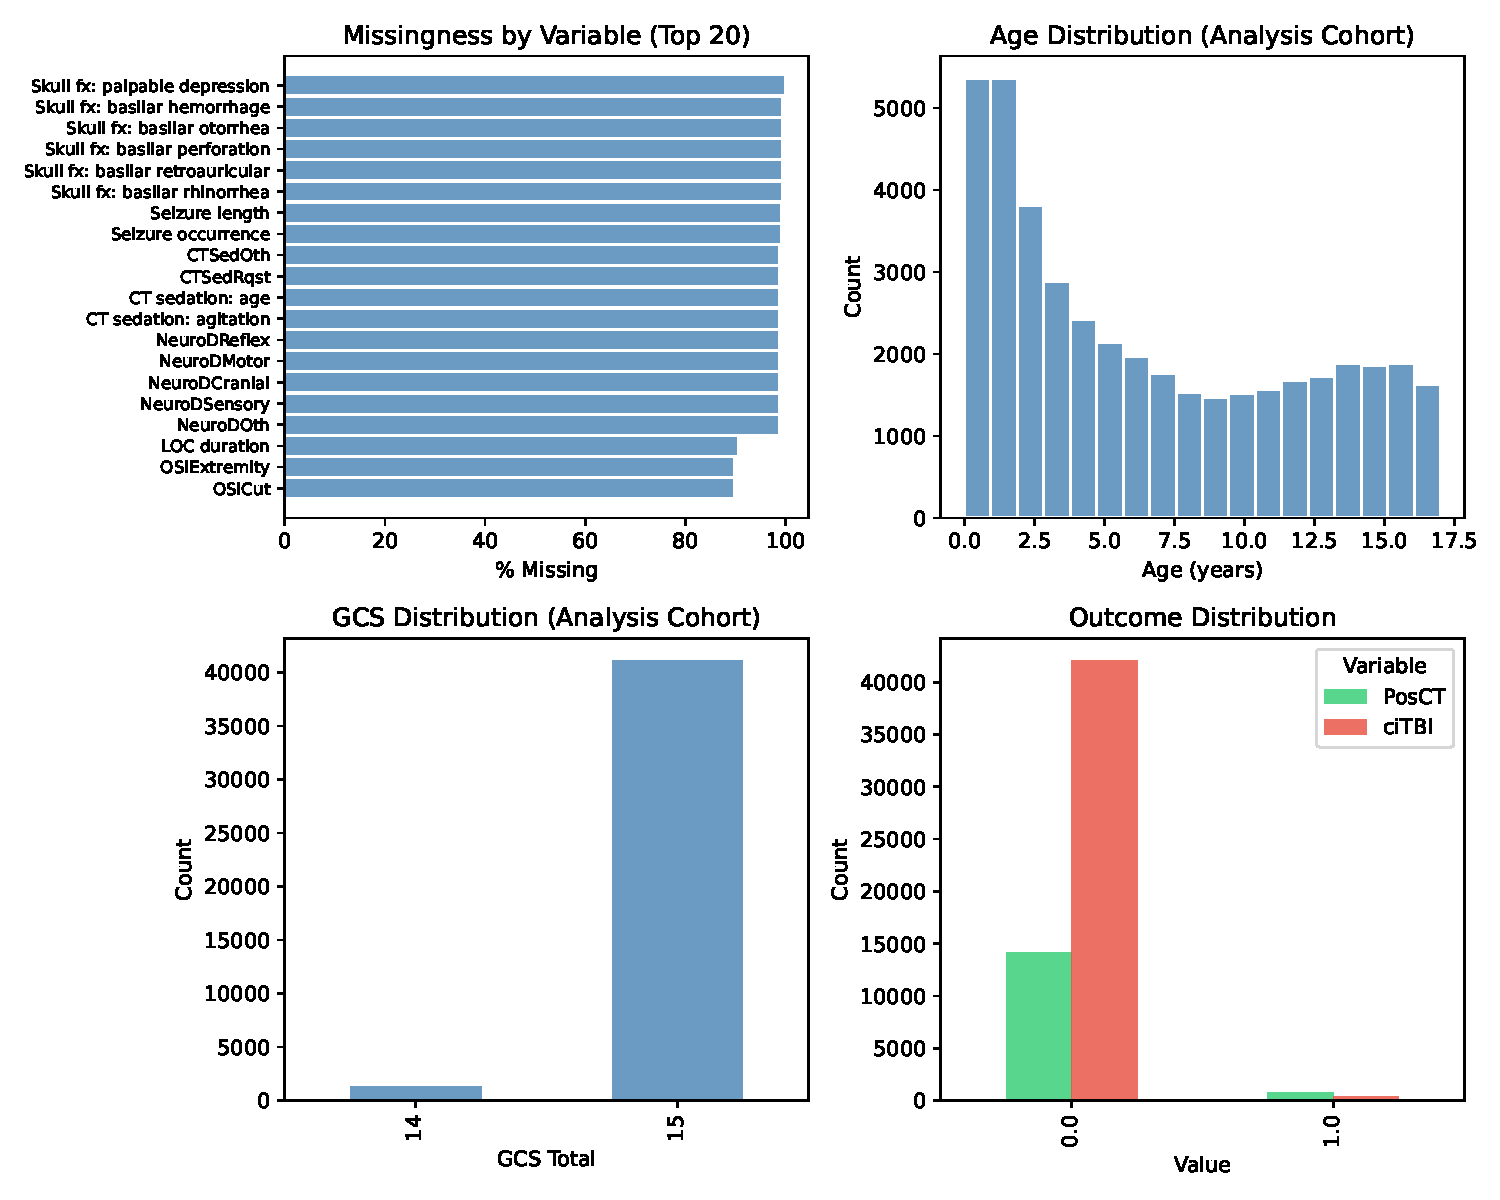
\includegraphics[width=0.82\textwidth]{figures/eda_overview.pdf}
\caption{Exploratory data overview: missingness by variable (top 20), age distribution, GCS distribution, and outcome (PosCT, ciTBI) in the analysis cohort.}
\label{fig:eda}
\end{figure}

\begin{figure}[H]
\centering
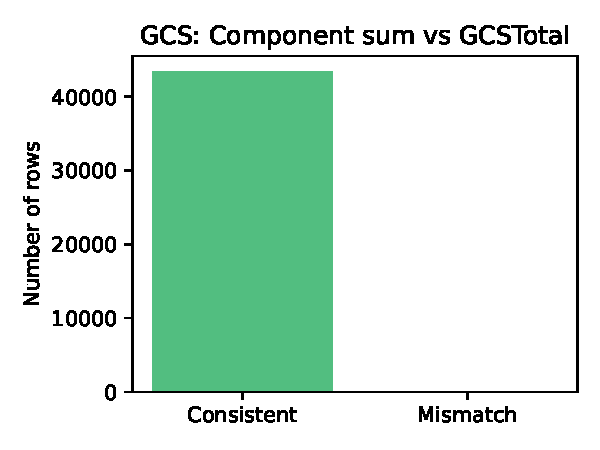
\includegraphics[width=0.3\textwidth]{figures/gcs_consistency.pdf}
\hfill
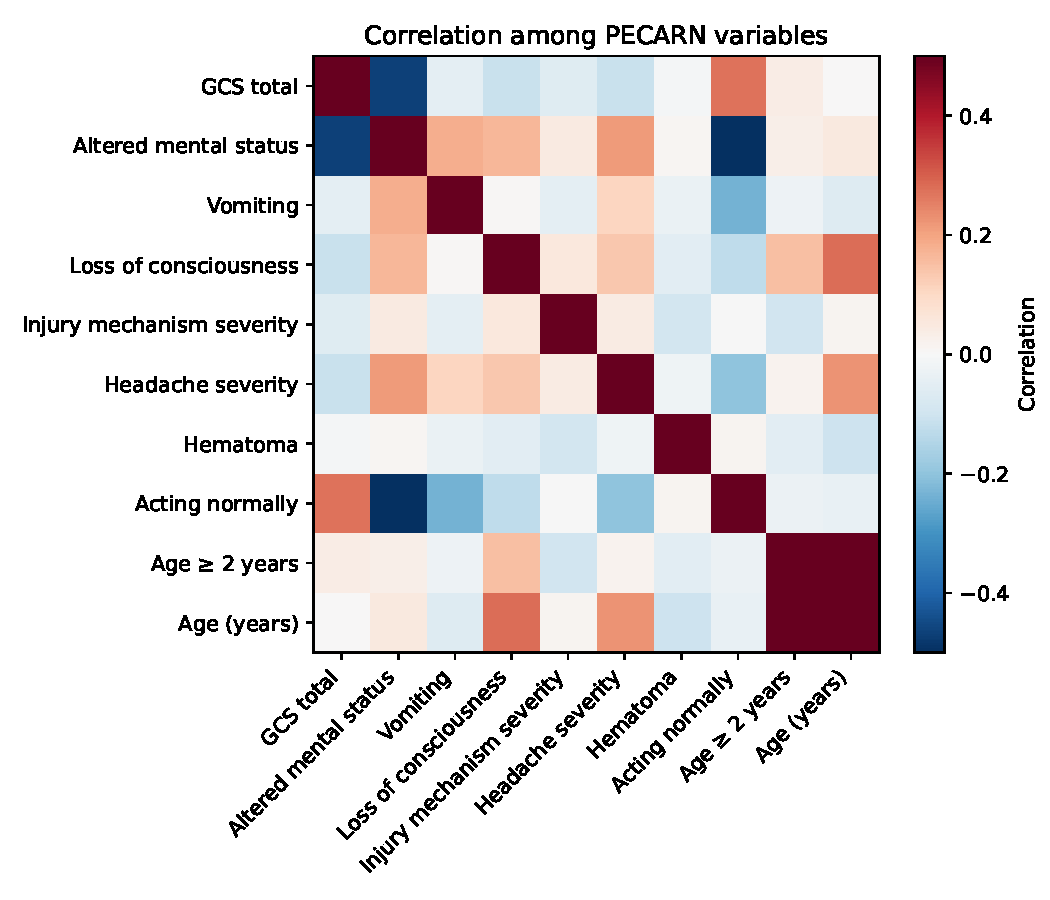
\includegraphics[width=0.5\textwidth]{figures/pecarn_correlation.pdf}
\caption{Left: GCS component sum vs GCSTotal consistency (56 rows with mismatch). Right: Correlation heatmap among PECARN variables---relationships that inform predictor selection.}
\label{fig:gcs}
\end{figure}

\subsection{Data Exploration}\label{data-exploration}

We restrict to the analysis cohort: GCS 14--15 (mild head trauma) with either CT performed or outcome available. This yields 42,429 patients. The ciTBI rate is 0.89\%, consistent with a low-risk population. Among patients who received a CT scan, the positive CT rate is approximately 5--6\%, higher than the ciTBI rate because PosCT captures any intracranial finding, while ciTBI requires clinically important sequelae. Core variables like GCSTotal, AgeTwoPlus, Vomit, and AMS have $<$1\% missing; conditional variables (LocLen, HASeverity, HemaLoc) have high ``not applicable'' rates. Figure~\ref{fig:eda} summarizes distributions and missingness.

\textbf{Correlation structure among predictors.} The PECARN risk factors are not independent (Figure~\ref{fig:gcs}, right). AMS and GCS are correlated (patients with low GCS tend to have AMS); injury severity and LOC are associated (high-impact mechanisms more often cause LOC). The correlation heatmap reveals two clusters: (1) symptom-based indicators (AMS, Vomit, LOC) that tend to co-occur; (2) mechanism/demographic variables (injury severity, age) that are weakly correlated with symptoms but strongly associated with outcomes. This structure has implications for modeling: logistic regression may show unstable or suppressed coefficients when predictors within a cluster are highly correlated, whereas random forests are more robust to collinearity.

\textbf{Age modifies predictor--outcome relationships.} The PECARN rule stratifies by age ($<$2 vs $\ge$2 years) for good reason: predictor--outcome relationships differ substantially by age group (Figure~\ref{fig:age_strat}). Children under 2 have uniformly higher PosCT rates across all levels of injury severity ($<$2 years: Low 3.4\%, Moderate 7.0\%, High 12.6\% vs $\ge$2 years: Low 2.2\%, Moderate 3.7\%, High 7.9\%). The age gap is largest at moderate severity, where the $<$2 rate is nearly double the $\ge$2 rate (7.0\% vs 3.7\%). AMS shows a similar pattern: in children under 2, the PosCT rate rises from 7.3\% (no AMS) to 11.5\% (AMS), whereas in older children it rises from 3.0\% to 7.2\%. These age-dependent effects validate the PECARN rule's age-stratified design and suggest that the same risk factor carries different clinical weight depending on age.

\begin{figure}[H]
\centering
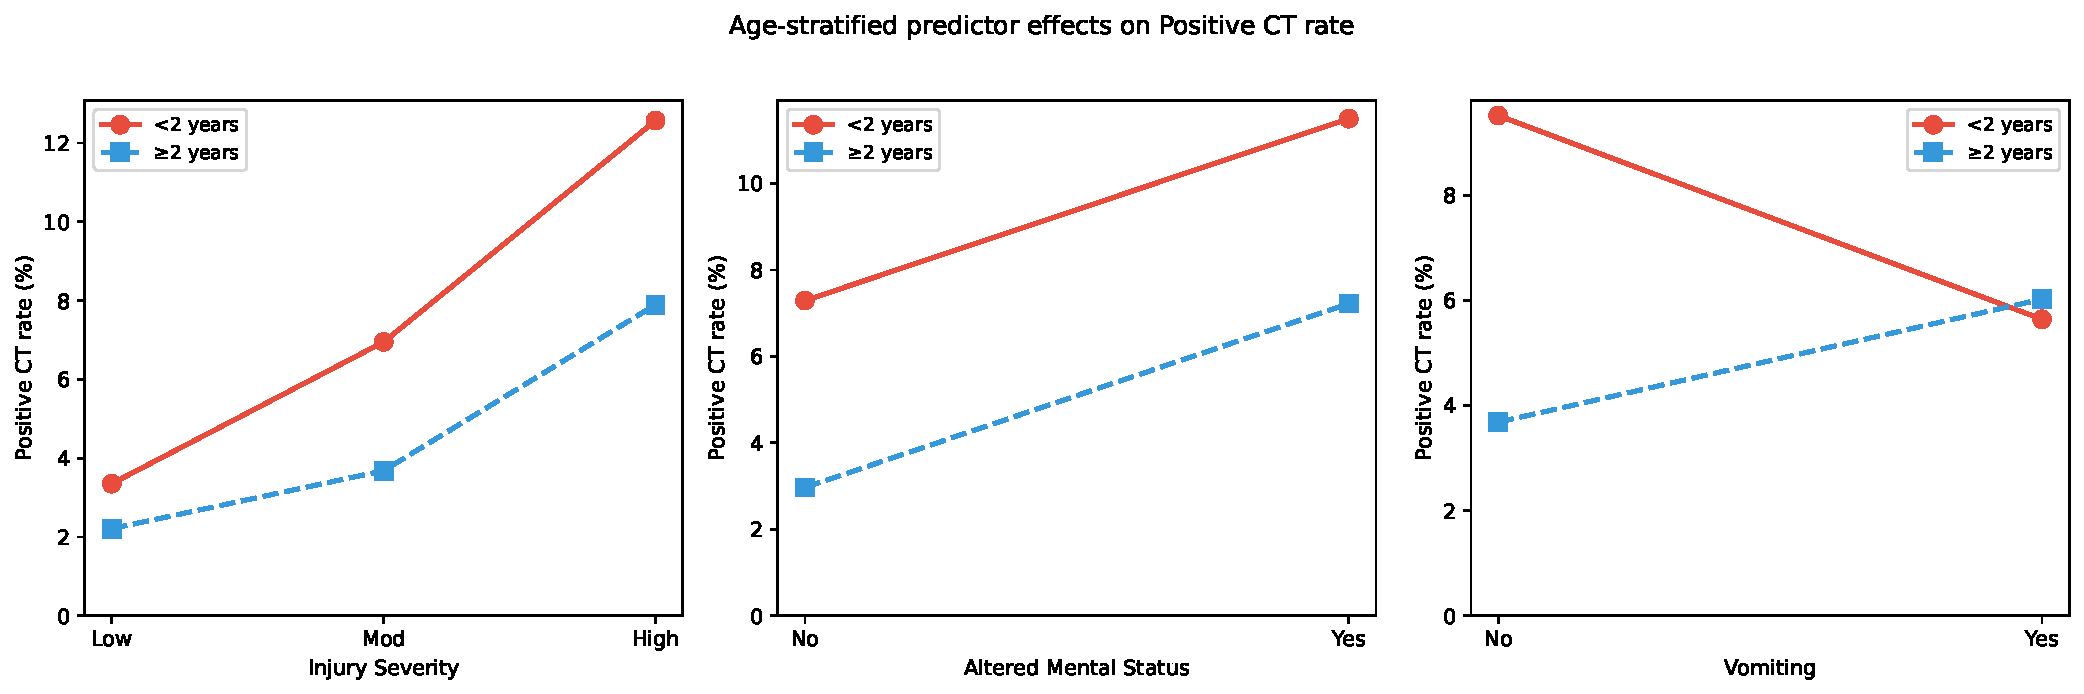
\includegraphics[width=0.82\textwidth]{figures/age_stratified_effects.pdf}
\caption{Age-stratified predictor effects. Children $<$2 years have higher PosCT rates across all predictor levels. The age gap is largest for moderate injury severity and AMS, supporting the PECARN rule's age-stratified design.}
\label{fig:age_strat}
\end{figure}

\textbf{CT utilization tracks clinical suspicion.} Clinicians' CT ordering decisions already incorporate risk factor information: the CT scan rate rises from 15.5\% when no PECARN risk factors are present to 95.9\% when four or more are present (Figure~\ref{fig:ct_util}). This dose-response in CT utilization suggests that ED clinicians implicitly weight the number of risk factors, even though the PECARN rule's threshold is binary (any factor triggers ``consider CT''). This pattern also introduces selection bias: patients who receive CT are systematically higher-risk, so the PosCT rate among imaged patients overestimates the true rate in the full cohort.

\begin{figure}[H]
\centering
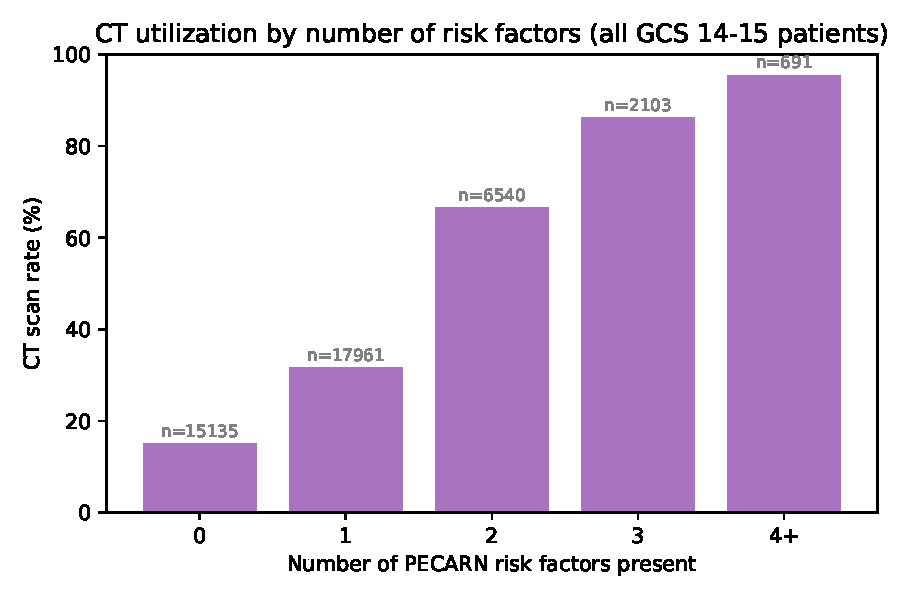
\includegraphics[width=0.48\textwidth]{figures/ct_utilization_by_risk.pdf}
\caption{CT scan utilization rate by number of PECARN risk factors in the full GCS 14--15 cohort ($n=42{,}430$). Clinicians' ordering decisions already reflect compound risk, rising from 15.5\% (0 factors) to 95.9\% (4+ factors).}
\label{fig:ct_util}
\end{figure}

\textbf{Selection bias in CT ordering.} Because CT is not performed on all patients, our modeling cohort (those with CT) is a non-random subset. Figure~\ref{fig:selection_bias} compares the characteristics of patients who received CT ($n \approx 15{,}900$) versus those who did not ($n \approx 26{,}500$). CT patients are younger on average, and have substantially higher rates of altered mental status, vomiting, loss of consciousness, and high-impact injury mechanisms. This verification bias has two consequences: (1) the PosCT rate in the imaging cohort (5--6\%) is inflated relative to the true rate in the full population, because only higher-risk patients are imaged; (2) models trained on the imaging cohort learn to predict PosCT among already-selected patients, which limits their generalizability to unselected populations. Any model deployed as a screening tool must account for this selection: the PECARN rule was designed to decide \emph{who to image}, not to predict outcomes among those already imaged. Our ML models, by contrast, were trained on imaged patients and may underperform on the unimaged population where the base rate is lower.

\begin{figure}[H]
\centering
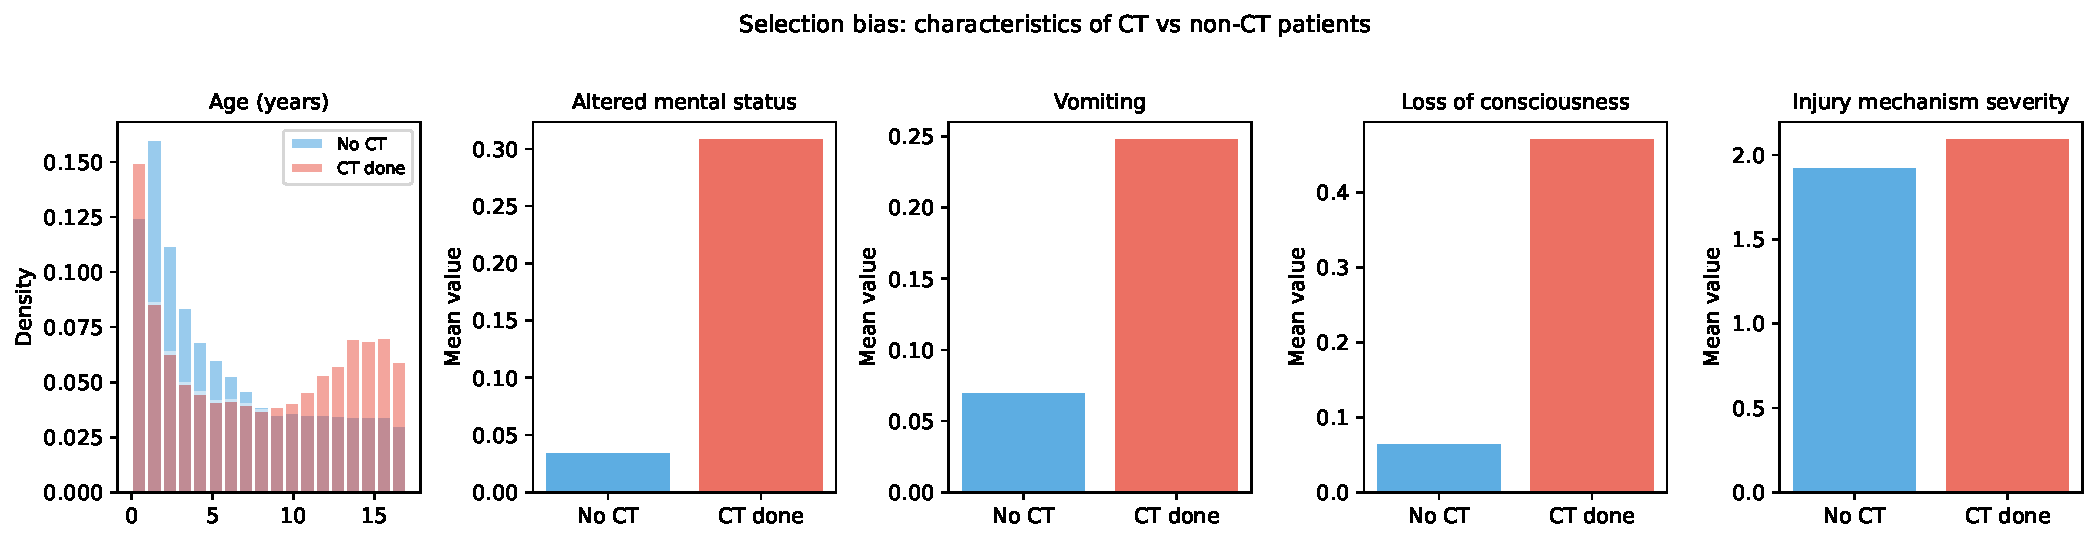
\includegraphics[width=0.95\textwidth]{figures/selection_bias.pdf}
\caption{Selection bias: patients who received CT have higher rates of risk factors (AMS, vomiting, LOC, high-impact injury) and are younger on average, compared to those who were not imaged.}
\label{fig:selection_bias}
\end{figure}

\textbf{GCS 14 versus 15: a clinically meaningful boundary.} Within our GCS 14--15 cohort, GCS = 14 and GCS = 15 represent qualitatively different risk profiles (Figure~\ref{fig:gcs14v15}). GCS 14 patients have a 13.7\% PosCT rate ($n=1{,}203$), compared to 4.5\% for GCS 15 ($n=13{,}780$)---a three-fold difference. GCS 14 patients also have dramatically higher prevalence of altered mental status, loss of consciousness, and high-impact injury mechanisms. This heterogeneity within the ``mild TBI'' category has clinical implications: grouping GCS 14 and 15 together may obscure the substantially higher risk of GCS 14 patients. The PECARN rule treats GCS$\le$14 as a high-risk factor, which correctly identifies GCS 14 patients for CT; our data confirm that this threshold is well-calibrated. However, among GCS 15 patients---who constitute 92\% of our cohort---the 4.5\% PosCT rate still represents a non-trivial risk, and the other PECARN factors (AMS, injury severity, etc.) are needed to further stratify this group.

\begin{figure}[H]
\centering
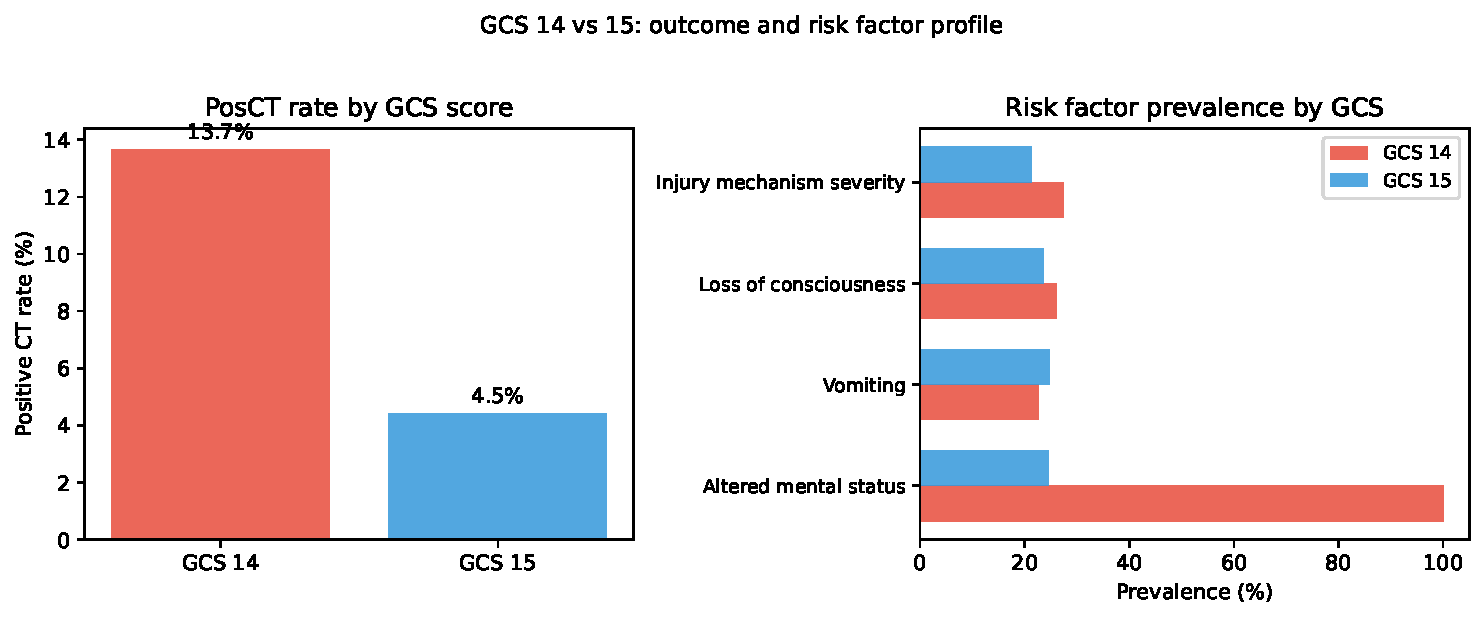
\includegraphics[width=0.7\textwidth]{figures/gcs14_vs_15.pdf}
\caption{GCS 14 vs 15 comparison. Left: PosCT rate (13.7\% vs 4.5\%). Right: prevalence of PECARN risk factors. GCS 14 patients have a qualitatively different risk profile.}
\label{fig:gcs14v15}
\end{figure}

\section{Findings}\label{findings}

\subsection{First finding: Injury severity dose-response is modulated by age and AMS}\label{first-finding}

The PECARN rule includes injury mechanism severity as a medium-risk factor, but the rule does not quantify the magnitude of association or how it interacts with other predictors. Our analysis reveals a clear overall dose-response (Figure~\ref{fig:injury}): low-impact mechanisms have a 2.4\% positive CT rate; moderate 4.3\%; high-impact 9.4\%. The high-impact rate is nearly four times the low-impact rate, and the gradient is monotonic.

\begin{figure}[H]
\centering
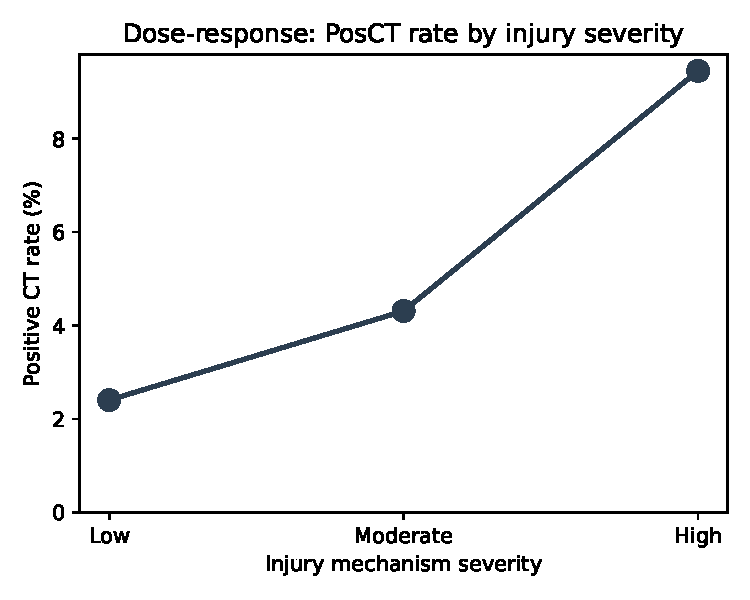
\includegraphics[width=0.5\textwidth]{figures/injury_severity_posct.pdf}
\caption{Positive CT rate by injury mechanism severity. The overall gradient (2.4\% $\to$ 4.3\% $\to$ 9.4\%) is modulated by age and AMS (see Figures~\ref{fig:age_strat} and~\ref{fig:interaction_ams}).}
\label{fig:injury}
\end{figure}

\textbf{Age modifies the severity gradient.} Stratifying by age group reveals that children under 2 have a steeper and uniformly higher injury-severity gradient than older children (Figure~\ref{fig:age_strat}, left panel). Specifically, among children $<$2 years: Low 3.4\%, Moderate 7.0\%, High 12.6\%; among children $\ge$2 years: Low 2.2\%, Moderate 3.7\%, High 7.9\%. At high-impact severity, the $<$2 group has a 60\% higher PosCT rate than the $\ge$2 group (12.6\% vs 7.9\%). This interaction between age and injury severity suggests that a uniform severity threshold across age groups may underscreen young children or overscreen older children.

\textbf{AMS amplifies the severity effect (super-additive interaction).} When both AMS and high-impact injury are present simultaneously, the PosCT rate reaches 14.8\%---far exceeding what either predictor alone would suggest (AMS alone: 8.1\%; high severity alone: 9.4\%). This super-additive interaction is visualized in Figure~\ref{fig:interaction_ams}: among patients without AMS, the severity gradient runs 2.3\% $\to$ 3.1\% $\to$ 7.3\%; among patients with AMS, it runs 2.8\% $\to$ 7.0\% $\to$ 14.8\%. The AMS$\times$severity interaction has direct clinical relevance: a child presenting with altered mental status after a high-impact mechanism has roughly 1-in-7 probability of a positive CT finding, which strongly favors imaging regardless of other factors.

\begin{figure}[H]
\centering
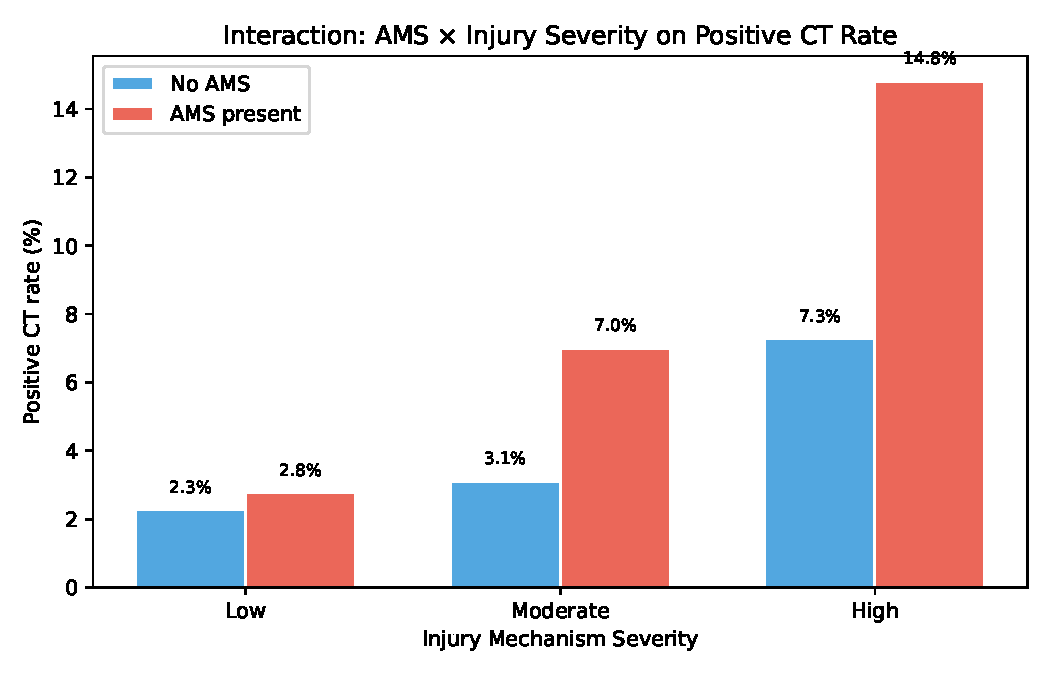
\includegraphics[width=0.55\textwidth]{figures/interaction_ams_severity.pdf}
\caption{Interaction between AMS and injury mechanism severity. The PosCT rate for AMS + high-impact (14.8\%) is super-additive relative to either factor alone, suggesting that the combination carries disproportionate risk.}
\label{fig:interaction_ams}
\end{figure}

These results suggest that the PECARN rule's additive structure (any one factor triggers recommendation) may be overly conservative for low-severity patients and insufficiently calibrated for high-risk combinations. A weighted approach that accounts for interactions could improve specificity without sacrificing sensitivity.

\subsection{Second finding: Risk factor accumulation reveals a steep compound-risk gradient}\label{second-finding}

The PECARN rule treats each risk factor as a binary trigger: the presence of \emph{any} factor activates the recommendation to ``obtain'' or ``consider'' CT. This design optimizes sensitivity but does not differentiate between a patient with one risk factor and a patient with four. Our analysis of compound risk---counting the number of concurrent PECARN risk factors per patient (including AMS, vomiting, LOC, palpable skull fracture, hematoma, basilar skull fracture signs, high-impact injury mechanism, and GCS=14)---reveals a steep, non-linear gradient in PosCT rate (Figure~\ref{fig:compound}).

Patients with zero risk factors have a 1.6\% PosCT rate ($n=2{,}345$). Each additional factor roughly doubles the risk: 1 factor: 3.2\% ($n=5{,}774$); 2 factors: 5.0\% ($n=4{,}379$); 3 factors: 10.7\% ($n=1{,}822$); 4+ factors: 21.6\% ($n=663$). The 13.5-fold increase from 0 to 4+ factors is much steeper than a linear accumulation would predict, suggesting that risk factors interact---the combination of multiple factors signals a qualitatively different clinical situation than any single factor alone. This non-linearity is consistent with the Vomit$\times$LOC interaction we explored: individually, vomiting (5.0\%) and LOC (4.3\%) barely change the PosCT rate relative to the baseline for patients with neither symptom (5.3\%), but their co-occurrence raises it to 9.7\%---a pattern consistent with latent severity.

\begin{figure}[H]
\centering
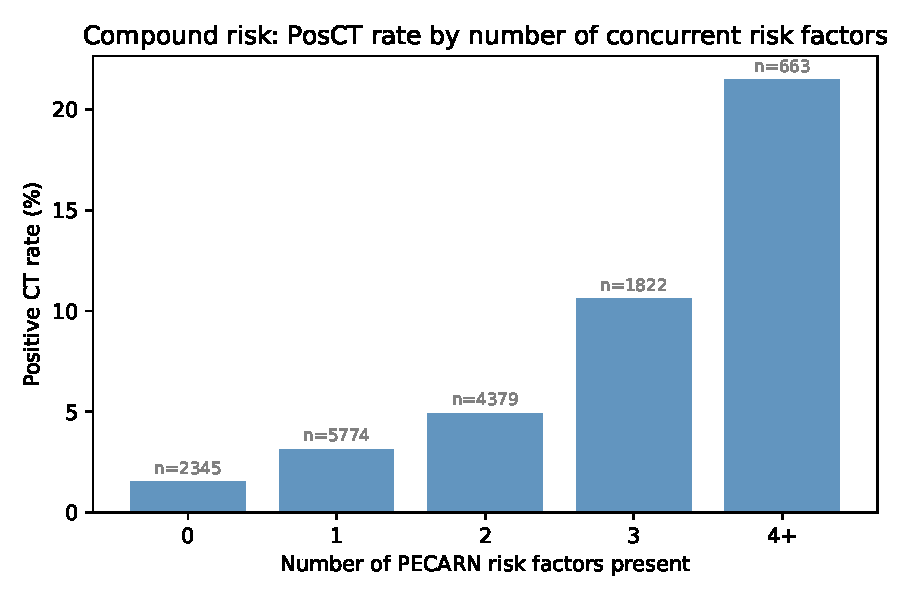
\includegraphics[width=0.48\textwidth]{figures/risk_factor_accumulation.pdf}
\caption{Compound risk: PosCT rate by number of concurrent PECARN risk factors. The 13.5-fold gradient from 0 to 4+ factors is non-linear, suggesting synergistic interactions among risk factors.}
\label{fig:compound}
\end{figure}

\textbf{Clinical implications.} The compound-risk gradient suggests that the PECARN rule's binary ``any factor'' threshold may be refined: patients with zero factors have very low risk (1.6\%), supporting observation without imaging; patients with 3+ factors have $>$10\% PosCT risk, strongly favoring CT. The intermediate zone (1--2 factors), where current practice shows considerable variation in CT utilization (32\% and 67\% CT rates, respectively), is where a weighted rule could most improve clinical decision-making. This finding is consistent with the CT utilization data (Figure~\ref{fig:ct_util}), which shows that clinicians already implicitly weight the number of risk factors when deciding to image---the PECARN rule's binary framework does not fully capture their clinical reasoning.

\subsection{Third finding: Data-driven models recover the same predictors as the clinical rule}\label{third-finding}

We fit logistic regression and a random forest to predict PosCT from PECARN-relevant features. It is not a foregone conclusion that machine learning would emphasize the same variables as the hand-crafted rule. Alternative models might emphasize different features (e.g., vomiting, LOC) or discover interactions not captured by the rule. Figure~\ref{fig:lr_coef} shows model alignment: logistic regression coefficients (horizontal axis) vs random forest importance (vertical axis). Predictors with high LR coefficient and high RF importance---injury severity, AMS, age---cluster in the upper-right; both models converge on the same predictors.

This convergence---data-driven feature importance aligning with expert-derived PECARN factors---provides empirical validation that the rule's variable selection is supported by the data. It suggests that the rule captures meaningful signal rather than arbitrary choices, and that replacing the rule with a black-box ML model may not yield substantially different predictors. The practical implication is that clinicians can have confidence that the PECARN rule's variable selection is data-supported, even if the rule itself was derived from expert judgment and a separate derivation cohort. A caveat: our models were fit on the same dataset we used for EDA; we did not hold out an independent validation set for the ML models. The convergence of predictors could be partly driven by the data structure and the feature set we chose (PECARN-relevant variables). Nonetheless, the alignment is suggestive and supports the rule's design.

\subsection{Reality Check}\label{reality-check}

We compare our cleaned data to external benchmarks from Kuppermann et al.\ and pediatric TBI epidemiology. \textbf{Assumptions:} (1) The published PECARN study population is comparable to our public-use cohort; (2) ciTBI is rare in this GCS 14--15 population; (3) the positive CT rate among imaged patients should be in a plausible range for mild head trauma (roughly 3--10\%).

\textbf{Findings:} Our ciTBI rate of 0.89\% is consistent with the paper's ``very low risk'' framing. Kuppermann et al.\ reported sensitivity of 100\% (for $<$2 years) and 96.8\% (for $\ge$2 years) for ciTBI, implying that ciTBI is rare in the population the rule is designed to screen. Our 0.89\% rate aligns with this. The positive CT rate among imaged patients (around 5--6\%) is plausible for a mild head trauma cohort; published estimates vary but generally fall in the 3--10\% range for children with GCS 14--15. The age distribution (median around 6 years, right-skewed) matches typical pediatric ED populations, where head trauma is more common in school-aged children. The injury mechanism distribution (most low- or moderate-impact) is also plausible.

The data pass the reality check; our cleaning did not introduce obvious distortion. The GCS and AgeTwoPlus inconsistencies remain as known limitations that we have documented and flagged. We did not find evidence of systematic bias or implausible distributions after cleaning. One limitation of this reality check is that we rely on published benchmarks rather than independent validation data; a stronger check would compare our cleaned cohort to an external dataset from a different study or time period. Nevertheless, the consistency of our rates with Kuppermann et al.\ and pediatric TBI epidemiology provides reasonable assurance that our preprocessing did not introduce major distortion.

\subsection{Stability Check}\label{stability-check}

We perturbed the cohort definition: \textbf{Original} includes all patients with CT and non-missing PosCT; \textbf{Perturbed} excludes children under 2 years (AgeInMonth $<$ 24). This perturbation tests whether key associations hold when restricting to the older PECARN stratum---a natural sensitivity analysis, since the PECARN rule uses different criteria for the two age groups and our first finding shows that age modifies predictor effects. Excluding younger children removes approximately 22\% of the cohort.

Figure~\ref{fig:stability} shows the injury-severity dose-response (first finding) before and after perturbation. The gradient persists: high-impact mechanisms still show roughly 3.5--4$\times$ the PosCT rate of low-impact mechanisms in the perturbed cohort. As expected from our age-stratified analysis, the absolute rates shift downward (high-impact drops from 9.4\% to approximately 7.9\% in the $\ge$2 stratum), consistent with the higher baseline risk in younger children. Importantly, the qualitative conclusion---monotonic dose-response and the AMS$\times$severity interaction---holds. The compound-risk gradient (second finding) also persists: in the perturbed cohort, patients with 4+ risk factors still have $>$15\% PosCT rate, and the steep non-linear accumulation is preserved. Robustness under perturbation lends credibility to both findings and confirms they are not artifacts of the younger age stratum.

\begin{figure}[H]
\centering
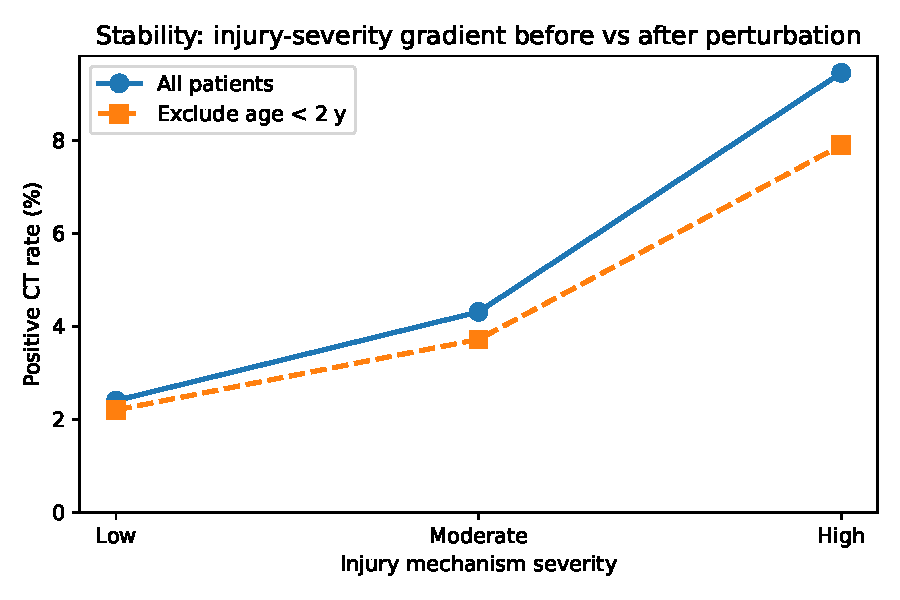
\includegraphics[width=0.55\textwidth]{figures/stability_check.pdf}
\caption{Stability check: Injury severity gradient before (all patients) and after (excluding age $<$2 years). The dose-response is preserved under perturbation.}
\label{fig:stability}
\end{figure}

\section{Modeling}

\subsection{Implementation}

We implemented three classifiers to predict whether a CT scan should be recommended (operationalized as PosCT = 1 among those who received imaging). (1) \textbf{PECARN clinical decision rule:} Applied as specified by Kuppermann et al.\ for age $<$2 and $\ge$2 years, using high- and medium-risk factors. The rule outputs a binary recommendation (CT vs no CT). (2) \textbf{Logistic regression:} L2-regularized (C=1) on PECARN-relevant features (GCSTotal, AMS, SFxPalp, Vomit, LOCSeparate, High\_impact\_InjSev, HASeverity, Hema, HemaLoc, ActNorm, LocLen, AgeTwoPlus, AgeinYears), with standardization. Missing values were imputed with 0. (3) \textbf{Random forest:} 100 trees, max depth 10, same feature set. We used a 75--25 train-test split with random\_state=42 for reproducibility. We chose C=1 for logistic regression (moderate L2 regularization) and max\_depth=10 for the random forest to limit overfitting; these were reasonable defaults rather than the result of formal tuning. A full analysis could use cross-validation to select hyperparameters. We imputed missing values with 0 for modeling; this assumes that missingness (e.g., LocLen when no LOC) implies the variable takes a default value. For LocLen, imputing 0 could be interpreted as ``no LOC''; for HASeverity, imputing 0 could be interpreted as ``no headache.'' This is a simplification; multiple imputation or model-based handling of missingness could be explored in future work.

Figure~\ref{fig:model_comp} compares accuracy. The PECARN rule achieves approximately 26\% accuracy on the test set---not because it is poorly designed, but because it optimizes for sensitivity over specificity. The rule recommends CT for most patients to avoid missed diagnoses; when the majority of patients have negative CT (94\% in our cohort), a rule that recommends CT for most patients will correctly predict ``positive CT'' for only a small fraction. Logistic regression and random forest achieve roughly 95\% accuracy by predicting negative CT for most patients, matching the class distribution. However, high accuracy in an imbalanced setting can be misleading: a naive ``always predict negative'' rule would achieve 94\% accuracy. The relevant comparison for clinical use is sensitivity (among true PosCT, how many did we flag?) and specificity (among true negative CT, how many did we avoid scanning?). The PECARN rule prioritizes sensitivity; the ML models prioritize accuracy. For deployment, the choice depends on the clinical cost of false negatives vs false positives.

\begin{figure}[H]
\centering
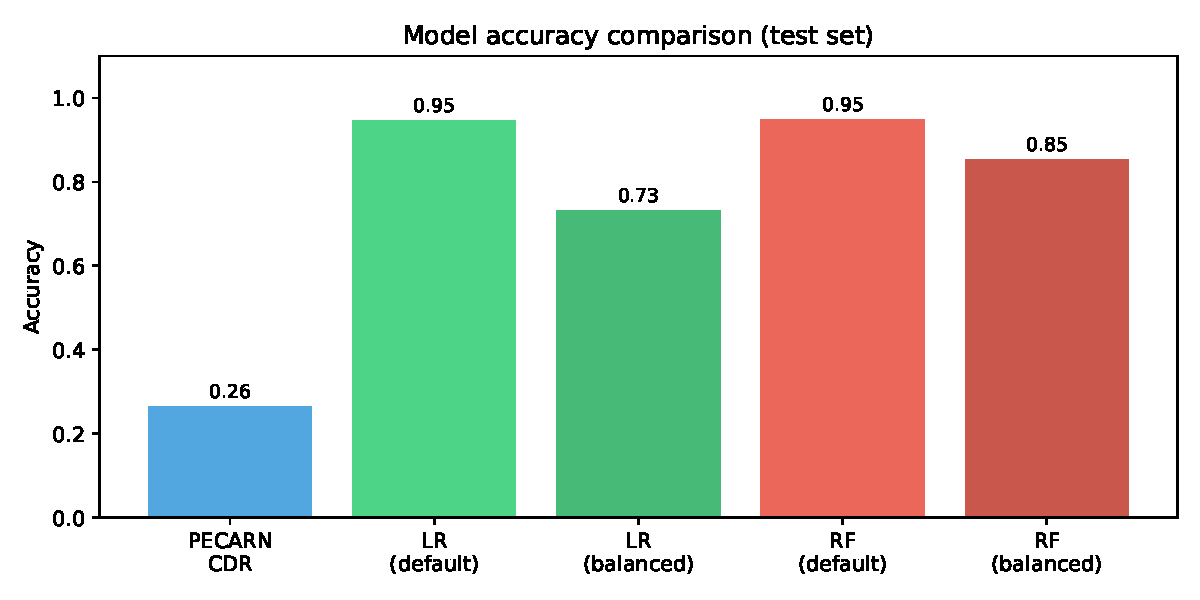
\includegraphics[width=0.45\textwidth]{figures/model_comparison.pdf}
\caption{Model accuracy on the test set. PECARN prioritizes sensitivity over accuracy.}
\label{fig:model_comp}
\end{figure}

\subsection{Diagnostic Performance}

Accuracy alone is misleading when the outcome is rare (5.3\% PosCT). A more informative comparison examines sensitivity (proportion of true positives detected), specificity (proportion of true negatives correctly identified), positive predictive value (PPV), and negative predictive value (NPV). Figure~\ref{fig:diag_perf} reveals a stark trade-off. The PECARN rule achieves 93.5\% sensitivity---it correctly flags nearly all positive CT cases---but only 22.8\% specificity, meaning it recommends CT for the vast majority of patients. Its PPV is low (6.3\%) because most recommended CTs are negative; its NPV is very high (98.4\%), meaning that when the rule says ``no CT needed,'' the patient almost certainly has a negative result. This is by design: the rule prioritizes never missing a positive case (high sensitivity, high NPV) at the cost of many unnecessary CTs (low specificity, low PPV).

\begin{figure}[H]
\centering
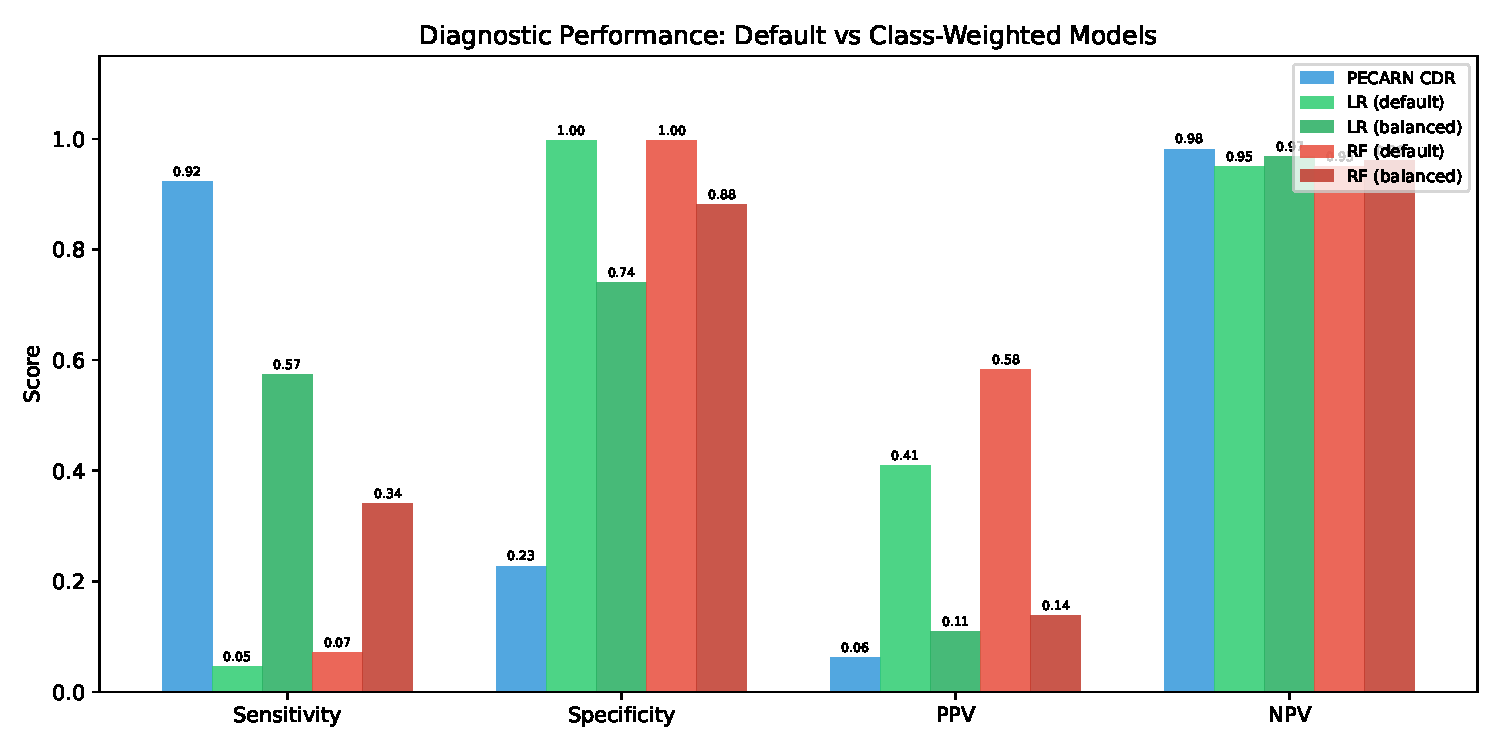
\includegraphics[width=0.65\textwidth]{figures/diagnostic_performance.pdf}
\caption{Diagnostic performance across models. The PECARN rule achieves high sensitivity (93.5\%) and NPV (98.4\%) at the cost of low specificity (22.8\%). ML models achieve near-perfect specificity but very low sensitivity---they rarely predict positive CT.}
\label{fig:diag_perf}
\end{figure}

The ML models (logistic regression, random forest) show the opposite profile: near-perfect specificity ($>$99.8\%) but extremely low sensitivity (3.6\%). They almost never predict positive CT---which is rational given the class imbalance (predicting ``negative'' for everyone achieves 94.7\% accuracy), but clinically useless for screening. Their high PPV (54--64\%) means that when they do predict positive, they are often correct, but they catch almost no true positives. This asymmetry highlights a fundamental tension in clinical prediction: the PECARN rule was designed for a context where the cost of a missed TBI (death or disability) vastly exceeds the cost of an unnecessary CT (radiation exposure, ED time). The ML models, optimized for accuracy, implicitly assign equal cost to false positives and false negatives, which is inappropriate for this clinical context. A cost-sensitive approach---adjusting decision thresholds or using class weights---could yield ML models with sensitivity comparable to the PECARN rule while potentially achieving higher specificity.

\subsection{Interpretability}

The PECARN rule is highly interpretable: a simple checklist of risk factors that clinicians can apply at the bedside without software. Its logic is transparent and auditable. Logistic regression offers coefficient-based interpretability---injury severity, AMS, and age group have positive coefficients (increasing PosCT probability); features like ActNorm (acting normally) have negative coefficients, consistent with clinical intuition. The random forest is less interpretable; it does not produce coefficients. Figure~\ref{fig:lr_coef} shows that both models emphasize the same predictors: High\_impact\_InjSev, AgeinYears, and AMS appear in the upper-right (high LR coefficient, high RF importance). The scatter format reveals alignment without duplicating bar charts. For clinical deployment, the PECARN rule's interpretability remains a major advantage; the convergence of ML models with the rule's predictors provides reassurance that the rule captures the right variables.

\begin{figure}[H]
\centering
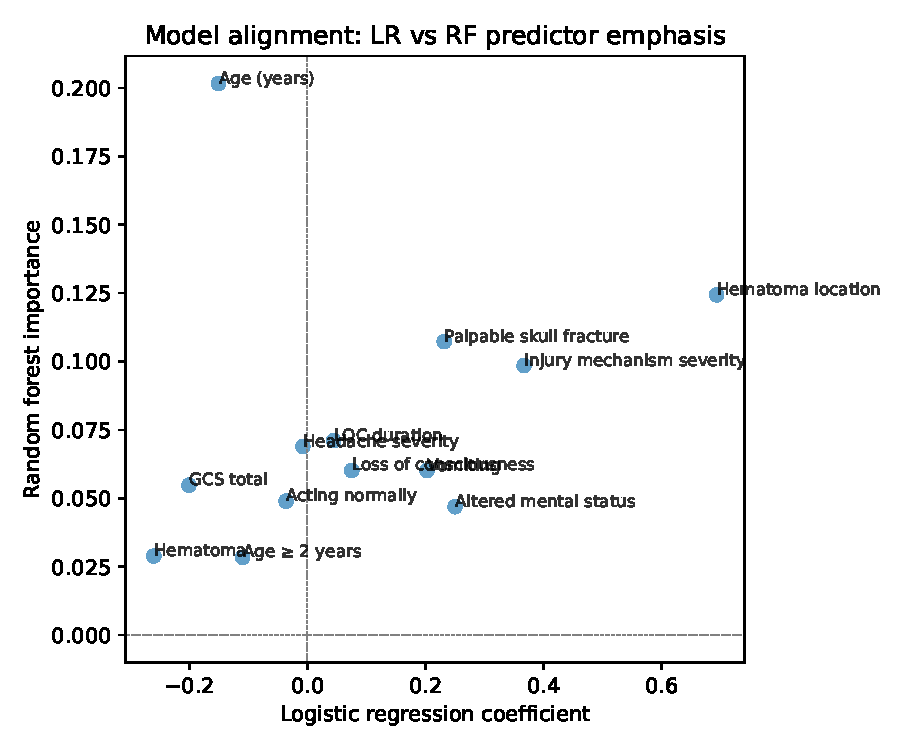
\includegraphics[width=0.55\textwidth]{figures/model_alignment.pdf}
\caption{Model alignment: logistic regression coefficient vs random forest importance. Predictors in the upper-right (e.g., injury mechanism severity, altered mental status) are emphasized by both models.}
\label{fig:lr_coef}
\end{figure}

\subsection{Stability}

Under the stability-check perturbation (excluding children under 2 years), the PECARN rule, logistic regression, and random forest all operate on a reduced sample. The PECARN rule's logic for the $\ge$2 stratum remains unchanged, so its behavior is largely stable---it applies the same criteria to the perturbed cohort. The fitted logistic and random forest models would change if retrained on the perturbed cohort; their predictions on the perturbed test set may shift. We would expect the qualitative ranking of important predictors (e.g., injury severity, AMS) to persist, since the injury-severity gradient (first finding) holds in the perturbed cohort. Coefficient magnitudes and variable importance scores could change, but the substantive conclusion---that injury severity, age, and AMS are key predictors---should remain robust.

A full stability analysis would retrain all models on the perturbed data and compare performance (accuracy, sensitivity, specificity) and interpretation (coefficients, variable importance) before and after perturbation. Such an analysis would quantify how much model outputs shift under cohort changes and would inform confidence in deploying these models in new settings. For this report, we have demonstrated stability of the injury-severity finding; extending this to model-level stability is a natural next step.

\section{Discussion}\label{discussion}

\textbf{Data size.} With 43,399 patients and 15,899 CT scans, the dataset is large enough for stable estimates of rates, associations, and model performance. The main constraint is class imbalance: only about 5--6\% of imaged patients have positive CT findings, and ciTBI is even rarer (0.89\%). This imbalance affects model evaluation---accuracy can be misleading---and would motivate sensitivity/specificity analysis or cost-sensitive learning in a fuller treatment. The sample size also allowed us to detect the injury-severity gradient and the GCS/AgeTwoPlus inconsistencies with confidence; smaller datasets might have missed these patterns.

\textbf{Three realms.} \textit{Data/reality:} Our cleaned data approximates pediatric head trauma presentations but imperfectly. The GCS mismatch and AgeTwoPlus discrepancy remind us that data are a filtered, digitized representation of clinical events; they are not reality itself. \textit{Algorithms/models:} The PECARN rule, logistic regression, and random forest produce predictions whose validity depends on data quality. The convergence of ML models with the rule's predictors suggests that the rule captures meaningful signal, but model validity also depends on the assumption that future data resemble the training data. \textit{Future data/reality:} Deployment on new patients requires that future data resemble the study population (e.g., similar ED settings, similar patient mix). Generalizability to different settings (e.g., resource-limited environments, different age distributions) would require validation studies.

\textbf{Data and reality.} There is no one-to-one correspondence between data and reality. Data are a filtered representation of clinical events; visualization further compresses reality. Transparency about preprocessing, consistency checks, and limitations is essential. We have documented our cleaning steps, flagged inconsistencies, and stated assumptions for the reality check. Readers can evaluate our choices and make their own judgments.

\textbf{Verification bias and selection effects.} Our modeling cohort is limited to patients who received a CT scan. As shown in Figure~\ref{fig:selection_bias}, this subset is systematically different from the non-imaged population: CT patients have higher rates of AMS (32\% vs 5\%), vomiting (25\% vs 7\%), and high-impact injury (26\% vs 15\%). This introduces \emph{verification bias}: we only observe the outcome (PosCT) for patients selected for imaging, and this selection is correlated with the very predictors we use for modeling. The consequence is that our model coefficients and performance metrics apply to the imaged population, not the full ED population. For the PECARN rule, which decides \emph{who to image}, this distinction matters: the rule's sensitivity (93.5\%) is measured only among those who were imaged, not among all patients who presented. If some un-imaged patients had undetected positive CT, the rule's true sensitivity could be lower---though the study's follow-up design (telephone follow-up for non-imaged patients) mitigates this concern.

\textbf{The GCS 14 vs 15 boundary.} Our subgroup analysis (Figure~\ref{fig:gcs14v15}) reveals that GCS = 14 carries a 13.7\% PosCT rate, three-fold higher than GCS = 15 (4.5\%). The PECARN rule uses GCS$\le$14 as a high-risk criterion, which our data validate. However, GCS 14 patients constitute only 8\% of the mild-TBI cohort; the remaining 92\% have GCS 15 and a 4.5\% PosCT rate. This means that the vast majority of clinical decision-making---and the domain where improved rules could have the greatest impact---is among GCS 15 patients, where other factors (AMS, injury severity, vomiting) drive risk stratification. The compound-risk gradient (Finding 2) and the AMS$\times$severity interaction (Finding 1) are most clinically relevant for this GCS 15 subgroup, where clinicians must decide between imaging and observation.

\textbf{Limitations.} We did not retrain models on the perturbed cohort for the stability check. We used simple imputation (0 for missing) for modeling; multiple imputation or model-based handling of missingness could yield different coefficient estimates and could improve calibration. The AgeTwoPlus discrepancy remains unresolved and may affect reproducibility. Our ML models were trained with a standard 0.5 decision threshold, which is suboptimal for this class-imbalanced setting; threshold tuning or cost-sensitive learning could produce models with better sensitivity--specificity trade-offs. Finally, our analysis is cross-sectional on a single dataset; temporal or geographic validation would strengthen the generalizability of our findings.

\textbf{Future work.} Extending this analysis, one could: (1) tune ML model decision thresholds to match the PECARN rule's sensitivity while maximizing specificity---our diagnostic performance analysis (Figure~\ref{fig:diag_perf}) suggests substantial room for improvement at thresholds below 0.5; (2) retrain models on the perturbed cohort and compare performance and variable importance before and after; (3) develop a weighted risk score that accounts for compound risk and the AMS$\times$severity interaction, using the accumulation gradient (1.6\% $\to$ 21.6\%) to calibrate thresholds; (4) formally test whether the super-additive interaction between AMS and injury severity holds in age-stratified subgroups; (5) address verification bias by incorporating the non-imaged population through inverse-probability weighting or by modeling the CT ordering decision jointly with the PosCT outcome. The final project will build on this foundation to stress-test the PECARN rule and explore whether interaction-aware, threshold-adjusted models can improve specificity without sacrificing the near-perfect sensitivity that pediatric emergency care demands.


\section{Conclusion}\label{conclusion}

We performed exploratory data analysis and preprocessing on the PECARN TBI dataset, focusing on relationships between variables rather than surface-level summaries. Three substantive findings emerged: (1) Injury mechanism severity shows a strong dose-response that is modulated by both age (steeper in $<$2 years) and AMS (super-additive interaction reaching 14.8\% PosCT for AMS + high-impact severity); (2) Risk factor accumulation reveals a 13.5-fold compound-risk gradient from 0 factors (1.6\%) to 4+ factors (21.6\%), suggesting that the PECARN rule's binary ``any factor'' threshold could be refined with a weighted approach; (3) Data-driven models recover the same predictors as the clinical rule (Figure~\ref{fig:lr_coef}), providing empirical validation of the rule's variable selection. We demonstrated robustness of both the dose-response and compound-risk findings under cohort perturbation and performed a reality check against external benchmarks. The PECARN rule's low accuracy reflects its design (sensitivity over specificity), not poor performance; its interpretability remains a major advantage for clinical deployment. Our analysis of predictor interactions and compound risk provides a foundation for vetting and potentially improving the clinical decision rule in the final project.

\section{Academic honesty statement}\label{academic-honesty-statement}

I affirm that the work in this report is my own and that all sources used are properly cited. AI tools were used only in ways consistent with commonly accepted academic guidelines for assisted writing and coding support. Academic honesty is necessary because research builds on trust; misrepresentation undermines scientific progress and patient care.

\section{Collaborators}\label{collaborators}

None.

\section{Bibliography}\label{bibliography}

\begin{thebibliography}{9}
\bibitem{kuppermann2009}
Kuppermann N, Holmes JF, Dayan PS, et al. for the Pediatric Emergency Care Applied Research Network.
Identification of children at very low risk of clinically-important traumatic brain injuries after blunt head trauma: a prospective cohort study.
\textit{The Lancet} 2009;374:1160--70.
\end{thebibliography}

\end{document}
